\documentclass[14pt]{beamer}
\usetheme{default}
\setbeamertemplate{navigation symbols}{} 
\setbeamertemplate{note page}[plain]

\definecolor{mygray}{gray}{0.1}

\usepackage{amsmath}

\DeclareMathOperator{\G}{G}
\DeclareMathOperator{\N}{N}
% \DeclareMathOperator{\Pr}{\Pr}
\DeclareMathOperator{\Uniform}{Uniform}

\usecolortheme[gray=0.2]{structure}

\setbeamertemplate{frametitle}
{
\begin{flushleft}
\textbf{\insertframetitle}
\end{flushleft}
}

\newcommand{\bi}{\begin{itemize}}
\newcommand{\ei}{\end{itemize}}

\usepackage{tgheros}

\title{\textbf{Bayesian Methods in Election Forecasting}}
\author{Michael Maltese \\ (Advisor: Gabriel Chandler)}
\date{November 1, 2013}

\begin{document}

\begin{frame}
\titlepage
\end{frame}

\begin{frame}[t]{Why'd we choose this?}
\bi
\item Nate Silver is cool. Got a lot of press during the 2012 election cycle
\item Other people doing it too! Princeton Election Consortium
\item Presumably math is interesting (turns out it is!)
\ei
\end{frame}

\begin{frame}[t]{Why is it important?}
\bi
\item Impress your friends
\item Journalists love it
\item But actually: \\ \begin{quote}\emph{Suppose you're a political campaign. How do you spend your money?}\end{quote}
\ei
\end{frame}

\begin{frame}[t]{Basic idea: polls}
\bi
\item National and by state
\item Run by tons of organizations (Gallup, Rasmussen, PPP, etc.)
\item Sort of accurate: Who's your sample? How do they know how they'll feel two months from now?
\item Biased: PPP literally makes up numbers if they feel like it! (liberal)
\ei
\end{frame}

\begin{frame}[t]{Problem: house biases}
You can:
\bi
\item Average all available polls.
\item Control for house biases: who leans left, who leans right, etc. Key part of FiveThirtyEight's model
\ei
\end{frame}

\begin{frame}
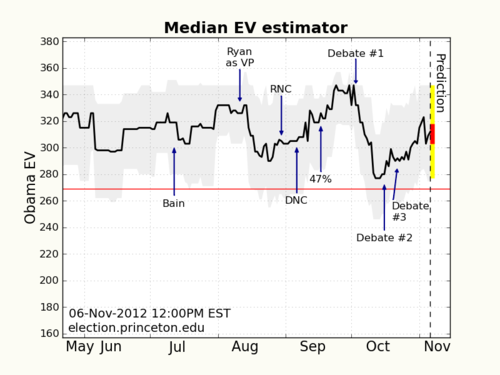
\includegraphics[width=\textwidth]{EV_history.png}
\end{frame}

\begin{frame}[t]{Problem: how reliable are polls in, say, February?}
\begin{itemize}
\item Not very.
\item You'd be better off forecasting from first principles, like: How is the economy? How many American soldiers are getting killed? (Hibbs 2008)
\end{itemize}
\end{frame}

\begin{frame}{Empirically}
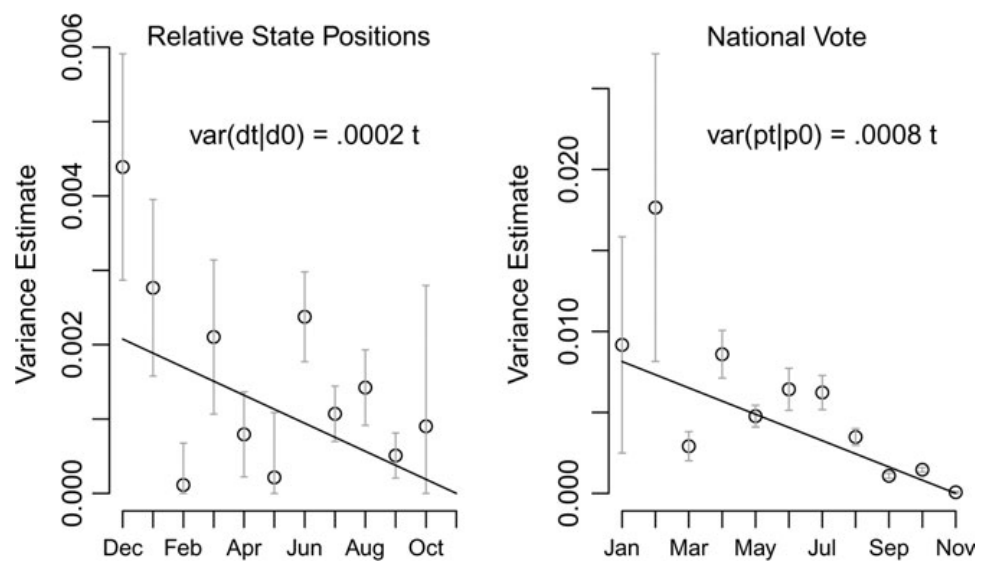
\includegraphics[width=\textwidth]{bayescombo_timevariance.png}
\end{frame}

\begin{frame}[t]{Theoretical: random walks}
Each time period, our preference changes by a draw from some normal random variable.

\[t_{i+1} \sim \N(t_i, \sigma^2)\]
\\[1em]
(Also cool because we can generate fake data!)
\end{frame}

\begin{frame}[t]{Solution: Bayesian inference}
Suppose it's May. How much do we believe the simple economic-growth-military-casualties forecast vs. the national polls?
\\[1em]
\emph{Bayesian inference}: update probability estimates using Bayes' rule

\[\Pr(A|B) = \frac{\Pr(B|A) \cdot \Pr(A)}{\Pr(B)}\]
\end{frame}

\begin{frame}[t]{National vs. state elections}
\bi
\item Popular vote means nothing!
\item Who wins the electoral college?
\item We need to forecast \emph{state} outcomes, not just national
\ei
\end{frame}

\begin{frame}[t]{Another motivation: Where do you put your money?}
\bi
\item Suppose again that you are a political campaign!
\item You want to spend your money where the vote will be close
\item It'd be awesome if we could predict where this happens
\ei
\end{frame}

\begin{frame}[t]{Forecasting states' votes}
\bi
\item Fun fact: states' deviation from the national vote is pretty stable
\item My suitemate:

\begin{quote}``Everyone looks at New York. Romney lost to 75\% Democratic. Bush lost to 60-something. Bush won the presidency, Romney didn't.''\end{quote}
\ei
\end{frame}

\begin{frame}{State stability}
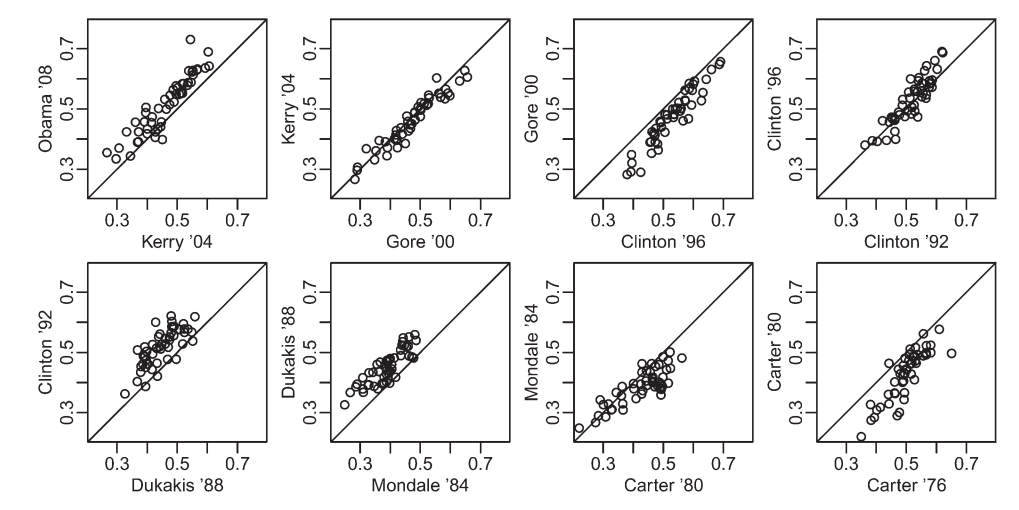
\includegraphics[width=\textwidth]{statestability.png}
\end{frame}

\begin{frame}[t]{Forecasting states' votes}
\bi
\item Guess before polls: they'll lean the same as in last election
\item Confidence based on how much they typically change between elections
\item Update based on state polls, based on time before Election Day as before
\ei
\end{frame}

\begin{frame}[t]{Further}
\bi
\item Why do people vote the way they do? (home-state advantage, etc.)
\item When are polls good? (Nate Silver has some tricky stuff)
\item Statistical tools: Gibbs sampling, Metropolis-Hastings algorithm, partial pooling, random walks
\item Applications in other realms: I found a cool paper on support for gay rights legislation.
\ei
\end{frame}

\begin{frame}
\begin{center}
{\Large\textbf{Congratulations, you've forecasted a presidential election}} \\[2em] Questions/Comments?
\end{center}
\end{frame}

\end{document}
